\problemname{Minecraft Speedrunning}
\noindent

\illustration{.3}{mcsr.png}{Filmklipp från Harrys Minecraft-speedrunning.}

Harry och hans vänner har på sistone börjar spela Minecraft tillsammans, och försöker klara av spelet så snabbt som möjligt.

Nu har Harrys gäng lyckats samla ihop alla resurser de behöver för att nå \textit{The Stronghold}, dit man behöver nå för att spelet ska kunna avslutas.

Positionerna mellan gängets nuvarande position och The Strongholds position kan modelleras på en tallinje, 
där Harrys gäng just nu befinner sig vid position $0$, och The Stronghold är beläget vid position $S$.

I Minecraft finns två världar: \textit{Overworld} och \textit{Nether}. Harrys gäng och The Stronghold befinner sig i Overworld.
Nether kan också modelleras som en tallinje, men alla koordinater är komprimerade med en faktor $8$:
en position $x$ i Nether motsvarar positionen $8x$ i Overworld.

Längs tallinjen i Nether finns $N$ förstörda \textit{Netherportaler}. Portal $i$ ligger vid position $x_i$ i Nether och leder till position $8x_i$ i Overworld.
För att kunna använda portal $i$ måste den först repareras, vilket tar $t_i$ sekunder. 
Notera att portalen behöver repareras oavsett om man går igenom från Overworld till Nether, eller Nether till Overworld.

Harrys gäng kan gå längs tallinjen i Overworld till valfri portalutgång (position $8x_i$) eller direkt till Stronghold vid position $S$.
Gånghastigheten är $1$, så det tar lika lång tid att gå som avståndet på tallinjen.

Vad är det minsta antalet sekunder det kan ta för Harrys gäng att nå The Stronghold från position $0$ i Overworld?

\section*{Indata}
Första raden innehåller två heltal $N$ och $S$ ($2 \le N \le 2 \cdot 10^5$), ($1 \le S \le 10^9$), antalet förstörda Netherportaler och positionen för The Stronghold i Overworld.

Varje av de följande $N$ raderna innehåller två heltal $x_i$ och $t_i$ ($1 \le x_i \le 10^9$, $8x_i < S$), ($1 \le t_i \le 10^9$), positionen för portal $i$ i Nether och tiden det tar att reparera portalen (i sekunder).

Det är garanterat att $x_i < x_{i+1}$ för alla $1 \le i < N$.

\section*{Utdata}
Skriv ut ett heltal, det minsta antalet sekunder det kan ta för Harrys gäng att nå The Stronghold från position $0$ i Overworld.


\section*{Poängsättning}
Din lösning kommer att testas på en mängd testfallsgrupper.
För att få poäng för en grupp så måste du klara alla testfall i gruppen.

\noindent
\begin{tabular}{| l | l | p{12cm} |}
  \hline
  \textbf{Grupp} & \textbf{Poäng} & \textbf{Gränser} \\ \hline
  $1$    & $15$        & $N = 2$ \\ \hline 
  $2$    & $19$        & $t_i = 1$ for all $i = 1, \dots, N$. \\ \hline 
  $3$    & $27$        & $N \le 1000$ \\ \hline
  $4$    & $39$        & Inga ytterligare begränsningar \\ \hline 
\end{tabular}

\section*{Förklaring av exempelfall 3}

\begin{figure}[h]
  \centering
  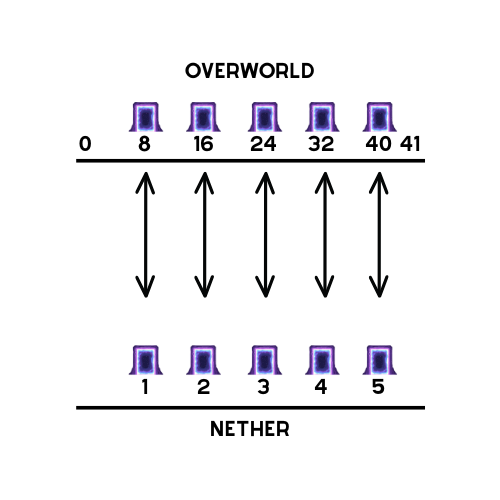
\includegraphics[width=0.6\linewidth]{fresh.png}
  \caption{Portaler enligt exempelfall 3.}
\end{figure}


Vi ser att det snabbaste sättet att nå The Stronghold är att gå
\begin{itemize}
  \item från position $0$ till position $16$ vid portal $2$, (tar $16$ sekunder),
  \item reparera portal $2$ och gå genom portal $2$ till position $2$ i Nether (tar $t_2 = 5$ sekunder),
  \item sedan gå till position $4$ i Nether (tar $2$ sekunder),
  \item reparera portal $4$ och gå igenom den (tar $t_4 = 5$ sekunder),
  \item och slutligen gå från position $32$ i Overworld till The Stronghold vid position $41$ (tar $9$ sekunder).
\end{itemize}

Totalt tar detta $16 + 5 + 2 + 5 + 9 = 37$ sekunder, vilket går att är det minsta möjliga.

